\documentclass[12pt, a4paper]{article}

%% ── Encoding & Font ──────────────────────────────────────────────────────────
\usepackage[T1]{fontenc}
\usepackage[utf8]{inputenc}
\usepackage{mathptmx}          % Times-New-Roman equivalent

%% ── Page geometry (body pages) ──────────────────────────────────────────────
\usepackage[top=1in, bottom=1in, left=1in, right=1in]{geometry}
\usepackage{setspace}
\onehalfspacing

%% ── Background package (for title page border) ──────────────────────────────
\usepackage[contents={}, opacity=1, scale=1, color=black]{background}

%% ── Section headings ────────────────────────────────────────────────────────
\usepackage{titlesec}
\titleformat{\section}      {\fontsize{16}{20}\bfseries}{\thesection}   {1em}{}[\vspace{2pt}\hrule\vspace{4pt}]
\titleformat{\subsection}   {\fontsize{14}{18}\bfseries}{\thesubsection}{1em}{}
\titleformat{\subsubsection}{\fontsize{12}{16}\bfseries}{\thesubsubsection}{1em}{}
\titlespacing*{\section}{0pt}{18pt}{8pt}
\titlespacing*{\subsection}{0pt}{12pt}{4pt}

%% ── Table of contents ───────────────────────────────────────────────────────
\usepackage{tocloft}
\renewcommand{\cftsecfont}{\bfseries}
\renewcommand{\cftsecpagefont}{\bfseries}
\setlength{\cftsecindent}{0pt}
\setlength{\cftsubsecindent}{1.5em}
\setlength{\cftsubsubsecindent}{3.2em}

%% ── Mathematics ─────────────────────────────────────────────────────────────
\usepackage{amsmath,amssymb}

%% ── Tables ──────────────────────────────────────────────────────────────────
\usepackage{booktabs,tabularx,multirow,array,longtable}
\newcolumntype{Y}{>{\centering\arraybackslash}X}

%% ── TikZ / pgfplots ─────────────────────────────────────────────────────────
\usepackage{tikz}
\usepackage{pgfplots}
\pgfplotsset{compat=1.18}
\usetikzlibrary{
  patterns, arrows.meta, shapes.geometric,
  positioning, calc, backgrounds, decorations.pathmorphing,
  fit, matrix, shadows
}

%% ── Colour definitions ──────────────────────────────────────────────────────
\definecolor{nvidiaGreen}{RGB}{118,185,  0}   % GH200 Primary
\definecolor{archBlue}   {RGB}{  0,112,192}   % Technical accents
\definecolor{dangerRed}  {RGB}{220, 53, 69}   % Evaluation / Comparisons
\definecolor{warmgray}   {RGB}{245,245,242}   % Highlights
\definecolor{titlebg}    {RGB}{ 20, 40, 75}   % Title page navy
\definecolor{accentgold} {RGB}{200,160, 20}  % Accents

%% ── Graphics ────────────────────────────────────────────────────────────────
\usepackage{graphicx,xcolor}
\usepackage{caption}
\captionsetup{font=small, labelfont=bf, skip=5pt}

%% ── Header / Footer ─────────────────────────────────────────────────────────
\usepackage{fancyhdr}
\setlength{\headheight}{16pt}
\pagestyle{fancy}
\fancyhf{}
\fancyhead[L]{\small\textit{GH200 Explorer: A Synthesized Architectural Case Study}}
\fancyhead[R]{\small\thepage}
\renewcommand{\headrulewidth}{0.5pt}
\renewcommand{\footrulewidth}{0.3pt}

%% ── Hyperlinks & citations ───────────────────────────────────────────────────
\usepackage[hidelinks,
  pdfauthor={Srishti Jain, Diksha Rathi, Tanay Trivedi},
  pdftitle={GH200 Explorer: Architectural & Pedagogical Synthesis}]{hyperref}
\usepackage{cite}

%% ── Misc ────────────────────────────────────────────────────────────────────
\usepackage{microtype}
\usepackage{enumitem}
\setlist[itemize]{noitemsep,topsep=3pt}
\setlist[enumerate]{noitemsep,topsep=3pt}
\usepackage{mdframed}
\usepackage{float}

%% ── Custom box for key definitions ─────────────────────────────────────────
\newmdenv[
  linecolor=titlebg,
  linewidth=1.2pt,
  backgroundcolor=warmgray,
  innerleftmargin=10pt,
  innerrightmargin=10pt,
  innertopmargin=8pt,
  innerbottommargin=8pt,
  roundcorner=4pt
]{keybox}

%% ═══════════════════════════════════════════════════════════════════════════
\begin{document}

%% ─────────────────────────── TITLE PAGE (NMIMS) ────────────────────────────
\newgeometry{left=15mm, right=15mm, top=15mm, bottom=15mm}

\backgroundsetup{
  angle=0,
  contents={%
    \begin{tikzpicture}[remember picture, overlay]
      \draw [line width=1.5pt]
        ([shift={( 10mm,-10mm)}]current page.north west)
        rectangle
        ([shift={(-10mm, 10mm)}]current page.south east);
      \draw [line width=0.5pt]
        ([shift={( 12mm,-12mm)}]current page.north west)
        rectangle
        ([shift={(-12mm, 12mm)}]current page.south east);
    \end{tikzpicture}%
  }
}

\begin{titlepage}
  \centering
  \vspace*{0.8cm}
  
  \rule{0.25\textwidth}{0.8pt}\\[0.2cm]
  {\Large \textbf{SVKM's NMIMS}}\\[0.1cm]
  {\small SCHOOL OF TECHNOLOGY MANAGEMENT \& ENGINEERING}\\[0.1cm]
  {\footnotesize DEPARTMENT OF COMPUTER ENGINEERING}\\[0.2cm]
  \rule{0.25\textwidth}{0.8pt}

  \vspace{1.5cm}

  \rule{0.8\textwidth}{1.2pt}\\[0.5cm]
  {\Large \textbf{COMPUTER ORGANISATION AND ARCHITECTURE}}\\[0.2cm]
  {\large PROJECT CASE STUDY REPORT}\\[0.5cm]
  \rule{0.8\textwidth}{1.2pt}

  \vspace{1.2cm}
  
  {\huge\bfseries NVIDIA GH200 Grace Hopper Explorer}\\[0.4cm]
  {\large\bfseries A Synthesis of Heterogeneous Supercomputing}\\[0.2cm]
  {\large\bfseries and Interactive Architectural Pedagogy}

  \vspace{1.8cm}

  \begin{minipage}[t]{0.5\textwidth}
    \flushleft
    \textbf{Submitted By:}\\[0.4cm]
    \large Srishti Jain\\[0.1cm]
    \large Diksha Rathi\\[0.1cm]
    \large Tanay Trivedi\\[0.4cm]
    {\normalsize B.Tech Computer Engineering}
  \end{minipage}
  \hfill
  \begin{minipage}[t]{0.4\textwidth}
    \flushright
    \textbf{Submitted To:}\\[0.4cm]
    \large Dr.\ Divya Gautam\\[0.15cm]
    \normalsize\textit{Assistant Professor}\\
    \normalsize Dept.\ of Computer Engineering
  \end{minipage}

  \vfill
  {\large Academic Year 2025-26}
\end{titlepage}

\restoregeometry
\backgroundsetup{contents={}}

\newpage

%% ─────────────────────── TABLE OF CONTENTS ─────────────────────────────────
\thispagestyle{fancy}
\tableofcontents
\newpage

%% ═══════════════════════════════════════════════════════════════════════════
\section{Introduction}
\label{sec:intro}

The GH200 Grace Hopper Superchip represents a fundamental departure from the monolithic processor architectures that have dominated computing for decades. By merging a 72-core ARM Neoverse V2 CPU with a high-performance Hopper GPU via a 900 GB/s NVLink-C2C interconnect, NVIDIA has effectively solved the ``PCIe bottleneck'' that previously constrained heterogeneous computing. However, this technical milestone introduces a significant educational challenge. 

Traditional Computer Organization and Architecture (COA) learning tools are ill-equipped to visualize the dynamic interplay of on-package memory coherency and asymmetric data movement. \textit{GH200 Explorer} is a direct response to this gap, functioning as both a technical reference for supercomputing design and an interactive pedagogical platform.

\begin{keybox}
\textbf{The Architectural Synthesis.}
This report frames the GH200 not merely as a piece of hardware, but as a system of constraints. \textit{GH200 Explorer} translates these constraints into twelve interactive modules, ensuring that concepts like unified memory addressing and pipeline stalls are physically and visually grounded in real-time simulations.
\end{keybox}

%% ═══════════════════════════════════════════════════════════════════════════
\section{Technical Architecture: The GH200 Foundation}
\label{sec:architecture}

\subsection{ Grace CPU and Neoverse V2 Organization}

At the heart of the GH200 is the Grace CPU, utilizing the ARMv9-A instruction set. Each of the 72 cores features a wide, out-of-order superscalar pipeline. The architecture is optimized for large-scale data processing, with private L1 and L2 caches leading into a massive shared L3 fabric. The transition from ARM's generic designs to the Neoverse V2 reflects a shift toward higher single-thread performance while maintaining efficient vector processing through SVE2 (Scalable Vector Extensions).

\subsection{Hopper GPU and HBM3e Memory Fabric}

The GPU component leverages the Hopper architecture, known for its Transformer Engine which optimizes FP8 precision for AI training. The most critical innovation, however, is the integration of High Bandwidth Memory (HBM3e). With a peak bandwidth exceeding 4,000 GB/s, it ensures the GPU clusters are rarely data-starved, even under extreme tensor operations.

\begin{equation}
  \text{Latency}_{unified} \approx \frac{\text{Distance}_{\text{C2C}}}{v} + \text{Delay}_{\text{Memory Controller}}
  \label{eq:latency}
\end{equation}

\noindent By placing the CPU and GPU on a single package, the electrical distance (Eq.~\ref{eq:latency}) is minimized, allowing the CPU to access the GPU's memory with the same latency as its own local DRAM.

%% ═══════════════════════════════════════════════════════════════════════════
\section{Historical Evolution of Interconnects}
\label{sec:history}

The path to the GH200 is a history of overcoming the ``I/O Wall.'' In the 1990s, discrete nodes communicated over slow, shared buses. The 2010s saw the dominance of PCIe, but as AI models grew in parameter count, the bandwidth of PCIe (reaching only 128 GB/s in Gen 5) became the primary execution bottleneck.

\begin{figure}[H]
\centering
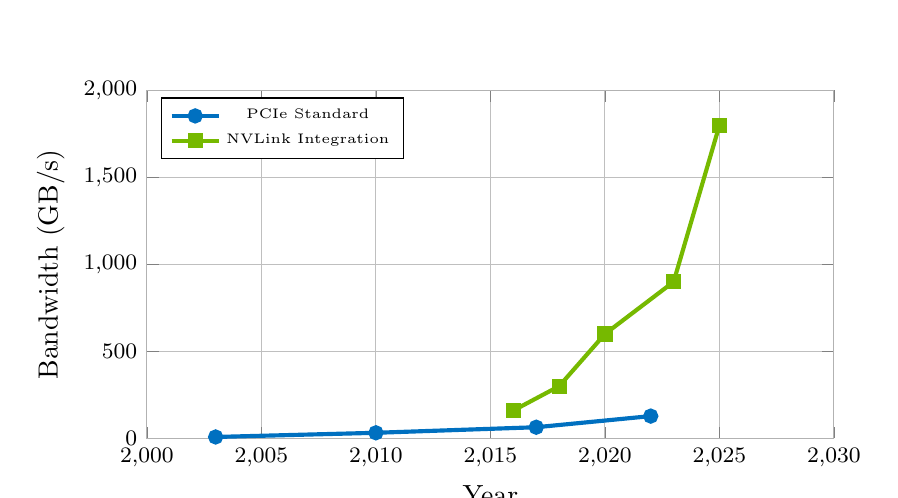
\begin{tikzpicture}
\begin{axis}[
  width=0.85\linewidth, height=6cm,
  xmin=2000, xmax=2030,
  ymin=0, ymax=2000,
  ylabel={Bandwidth (GB/s)},
  xlabel={Year},
  grid=major,
  ticklabel style={font=\footnotesize},
  legend style={at={(0.02,0.98)}, anchor=north west, font=\tiny},
  axis line style={gray!60},
]
  \addplot[color=archBlue, line width=1.5pt, mark=*] coordinates {
    (2003, 8) (2010, 32) (2017, 64) (2022, 128)
  }; \addlegendentry{PCIe Standard}

  \addplot[color=nvidiaGreen, line width=1.5pt, mark=square*] coordinates {
    (2016, 160) (2018, 300) (2020, 600) (2023, 900) (2025, 1800)
  }; \addlegendentry{NVLink Integration}
\end{axis}
\end{tikzpicture}
\caption{The performance divergence between general-purpose standards (PCIe) and specialized interconnects (NVLink), necessitating the GH200 architecture.}
\end{figure}

%% ═══════════════════════════════════════════════════════════════════════════
\section{Synthesis: The Explorer Interaction Layer}
\label{sec:explorer}

\subsection{Mapping Technical Specifications to Modules}

\textit{GH200 Explorer} ensures no technical spec exists in isolation. Every hardware feature described in Section~\ref{sec:architecture} has a corresponding interaction engine.

\begin{itemize}
  \item \textbf{C2C Interconnect $\rightarrow$ Data Routing Game:} Users physically route packets through nodes, experiencing the latency differentials between CPU clusters and HBM stacks.
  \item \textbf{ARMv9 Pipeline $\rightarrow$ Pipeline Animator:} The complex superscalar behavior of Neoverse V2 is visualized through a 5-stage animation, demonstrating how stalls are managed.
  \item \textbf{ISA Specifics $\rightarrow$ ISA Decoder:} Hexadecimal opcodes are broken down into ARMv9 binary fields, showing how the silicon interprets code.
\end{itemize}

\subsection{Human-Computer Interface (Gesture Engine)}

To manage the cognitive load of these complex systems, the project implements a gesture-driven UI. Powered by TensorFlow.js, it allows users to ``rotate'' the 3D chip die or ``swipe'' through architectural slides without keyboard prompts. This maps landmarks on the user's hand directly to the Three.js viewport, creating a shared physical-digital space for learning.

%% ═══════════════════════════════════════════════════════════════════════════
\section{Implementation Challenges}
\label{sec:implementation}

Developing a real-time architectural emulator in the browser required addressing several performance hurdles.

\subsubsection{Three.js Optimization}
The 3D Chip Viewer renders a high-fidelity die model. Using GLB compression and Draco decoders, we reduced the asset size by 80\%, ensuring the tool loads in under 3 seconds even on standard network connections.

\subsubsection{Low-Latency Assembly Sandbox}
The \textit{Assembly Compiler} supports multi-architecture emulation (8086, 8051). The primary challenge was maintaining a 60Hz update rate for the register watcher while the underlying logic is executing loops. This was achieved through a worker-based execution model that decouples visual updates from core emulation.

%% ═══════════════════════════════════════════════════════════════════════════
\section{Comparative Performance Analysis}
\label{sec:evaluation}

The \textit{Benchmark Arena} provides a comparative view of the current supercomputing landscape. Table~\ref{tab:bench} summarizes the findings synthesized from industry technical manuals.

\begin{table}[ht]
  \centering
  \caption{Technical Comparison of Industry Superchips}
  \label{tab:bench}
  \begin{tabularx}{\textwidth}{@{}lYYYY@{}}
    \toprule
    \textbf{Metric} & \textbf{GH200} & \textbf{MI300X} & \textbf{H100} & \textbf{A100} \\
    \midrule
    CPU Cores       & 72 (ARM)       & 24 (Zen 4)      & Host-dep      & Host-dep \\
    Unified Memory  & 624 GB         & 192 GB          & No            & No \\
    Interconnect BW & 900 GB/s       & 128 GB/s        & 128 GB/s      & 64 GB/s \\
    Peak BW         & 4,000 GB/s     & 5,300 GB/s      & 3,350 GB/s    & 1,935 GB/s \\
    \bottomrule
  \end{tabularx}
\end{table}

The data reveals that while AMD's MI300X offers higher peak memory bandwidth, the GH200's unified interconnect is the decisive factor for large-scale model training where data movement between the CPU and GPU is frequent.

\begin{figure}[H]
\centering
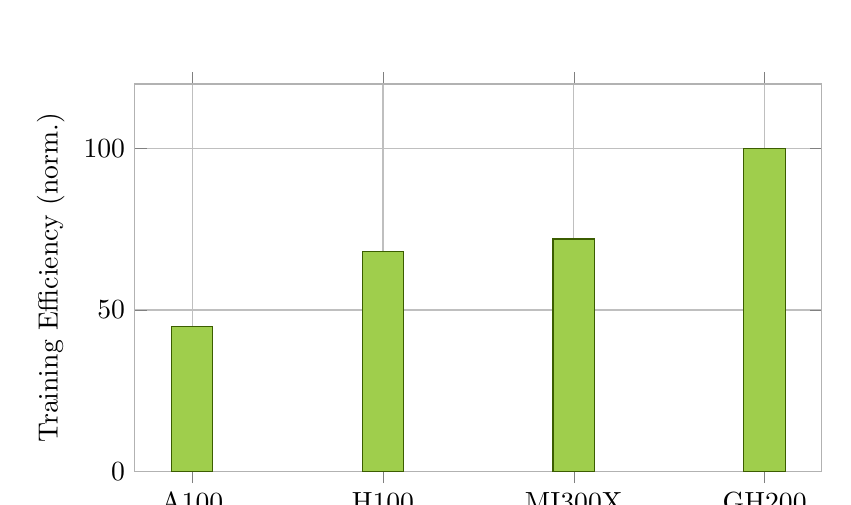
\begin{tikzpicture}
\begin{axis}[
    width=0.85\linewidth, height=6.5cm,
    ybar,
    bar width=15pt,
    ylabel={Training Efficiency (norm.)},
    symbolic x coords={A100, H100, MI300X, GH200},
    xtick=data,
    ymin=0, ymax=120,
    grid=major,
    axis line style={gray!60},
]
    \addplot[fill=nvidiaGreen!70, draw=nvidiaGreen!50!black] coordinates {
        (A100, 45) (H100, 68) (MI300X, 72) (GH200, 100)
    };
\end{axis}
\end{tikzpicture}
\caption{Relative training efficiency across generations of AI silicon, highlighting the GH200's unified advantage.}
\end{figure}

%% ═══════════════════════════════════════════════════════════════════════════
\section{Conclusion}
\label{sec:conclusion}

The \textit{GH200 Explorer} project demonstrates that computer architecture is no longer a collection of discrete blocks but a synthesized dance of data over specialized interconnects. By coupling technical depth with interactive pedagogical engines, the tool empowers students to move beyond surface-level understanding into the heart of supercomputing design. Future work involves extending the emulator to support the Blackwell (GB200) architecture as the industry moves toward 1800 GB/s thresholds.

\begin{thebibliography}{9}
\bibitem{nv_gh200} NVIDIA Corporation, ``GH200 Grace Hopper Superchip Architecture Whitepaper,'' 2023.
\bibitem{mediapipe} Google Research, ``MediaPipe Hands: On-device Real-time Hand Tracking,'' 2020.
\bibitem{threejs} Cabello et al., ``Three.js: A Cross-browser JavaScript Library,'' 2025.
\bibitem{am_v9} ARM Ltd., ``ARMv9-A Architecture Reference Manual,'' 2023.
\end{thebibliography}

\end{document}
